\documentclass{article}

\usepackage{graphicx}
\usepackage{amsmath}

\begin{document}

\title{Machine Learning Concepts}
\author{Gnkgo}
\date{\today}

\maketitle

\clearpage

\tableofcontents

\clearpage
% Convexity
\section{Convexity}
\begin{itemize}
    \item If $f$ is a differentiable convex function and $\nabla f(w) = 0$, then $w$ is the global minimum of $f$.
    \begin{figure}[h]
        \centering
        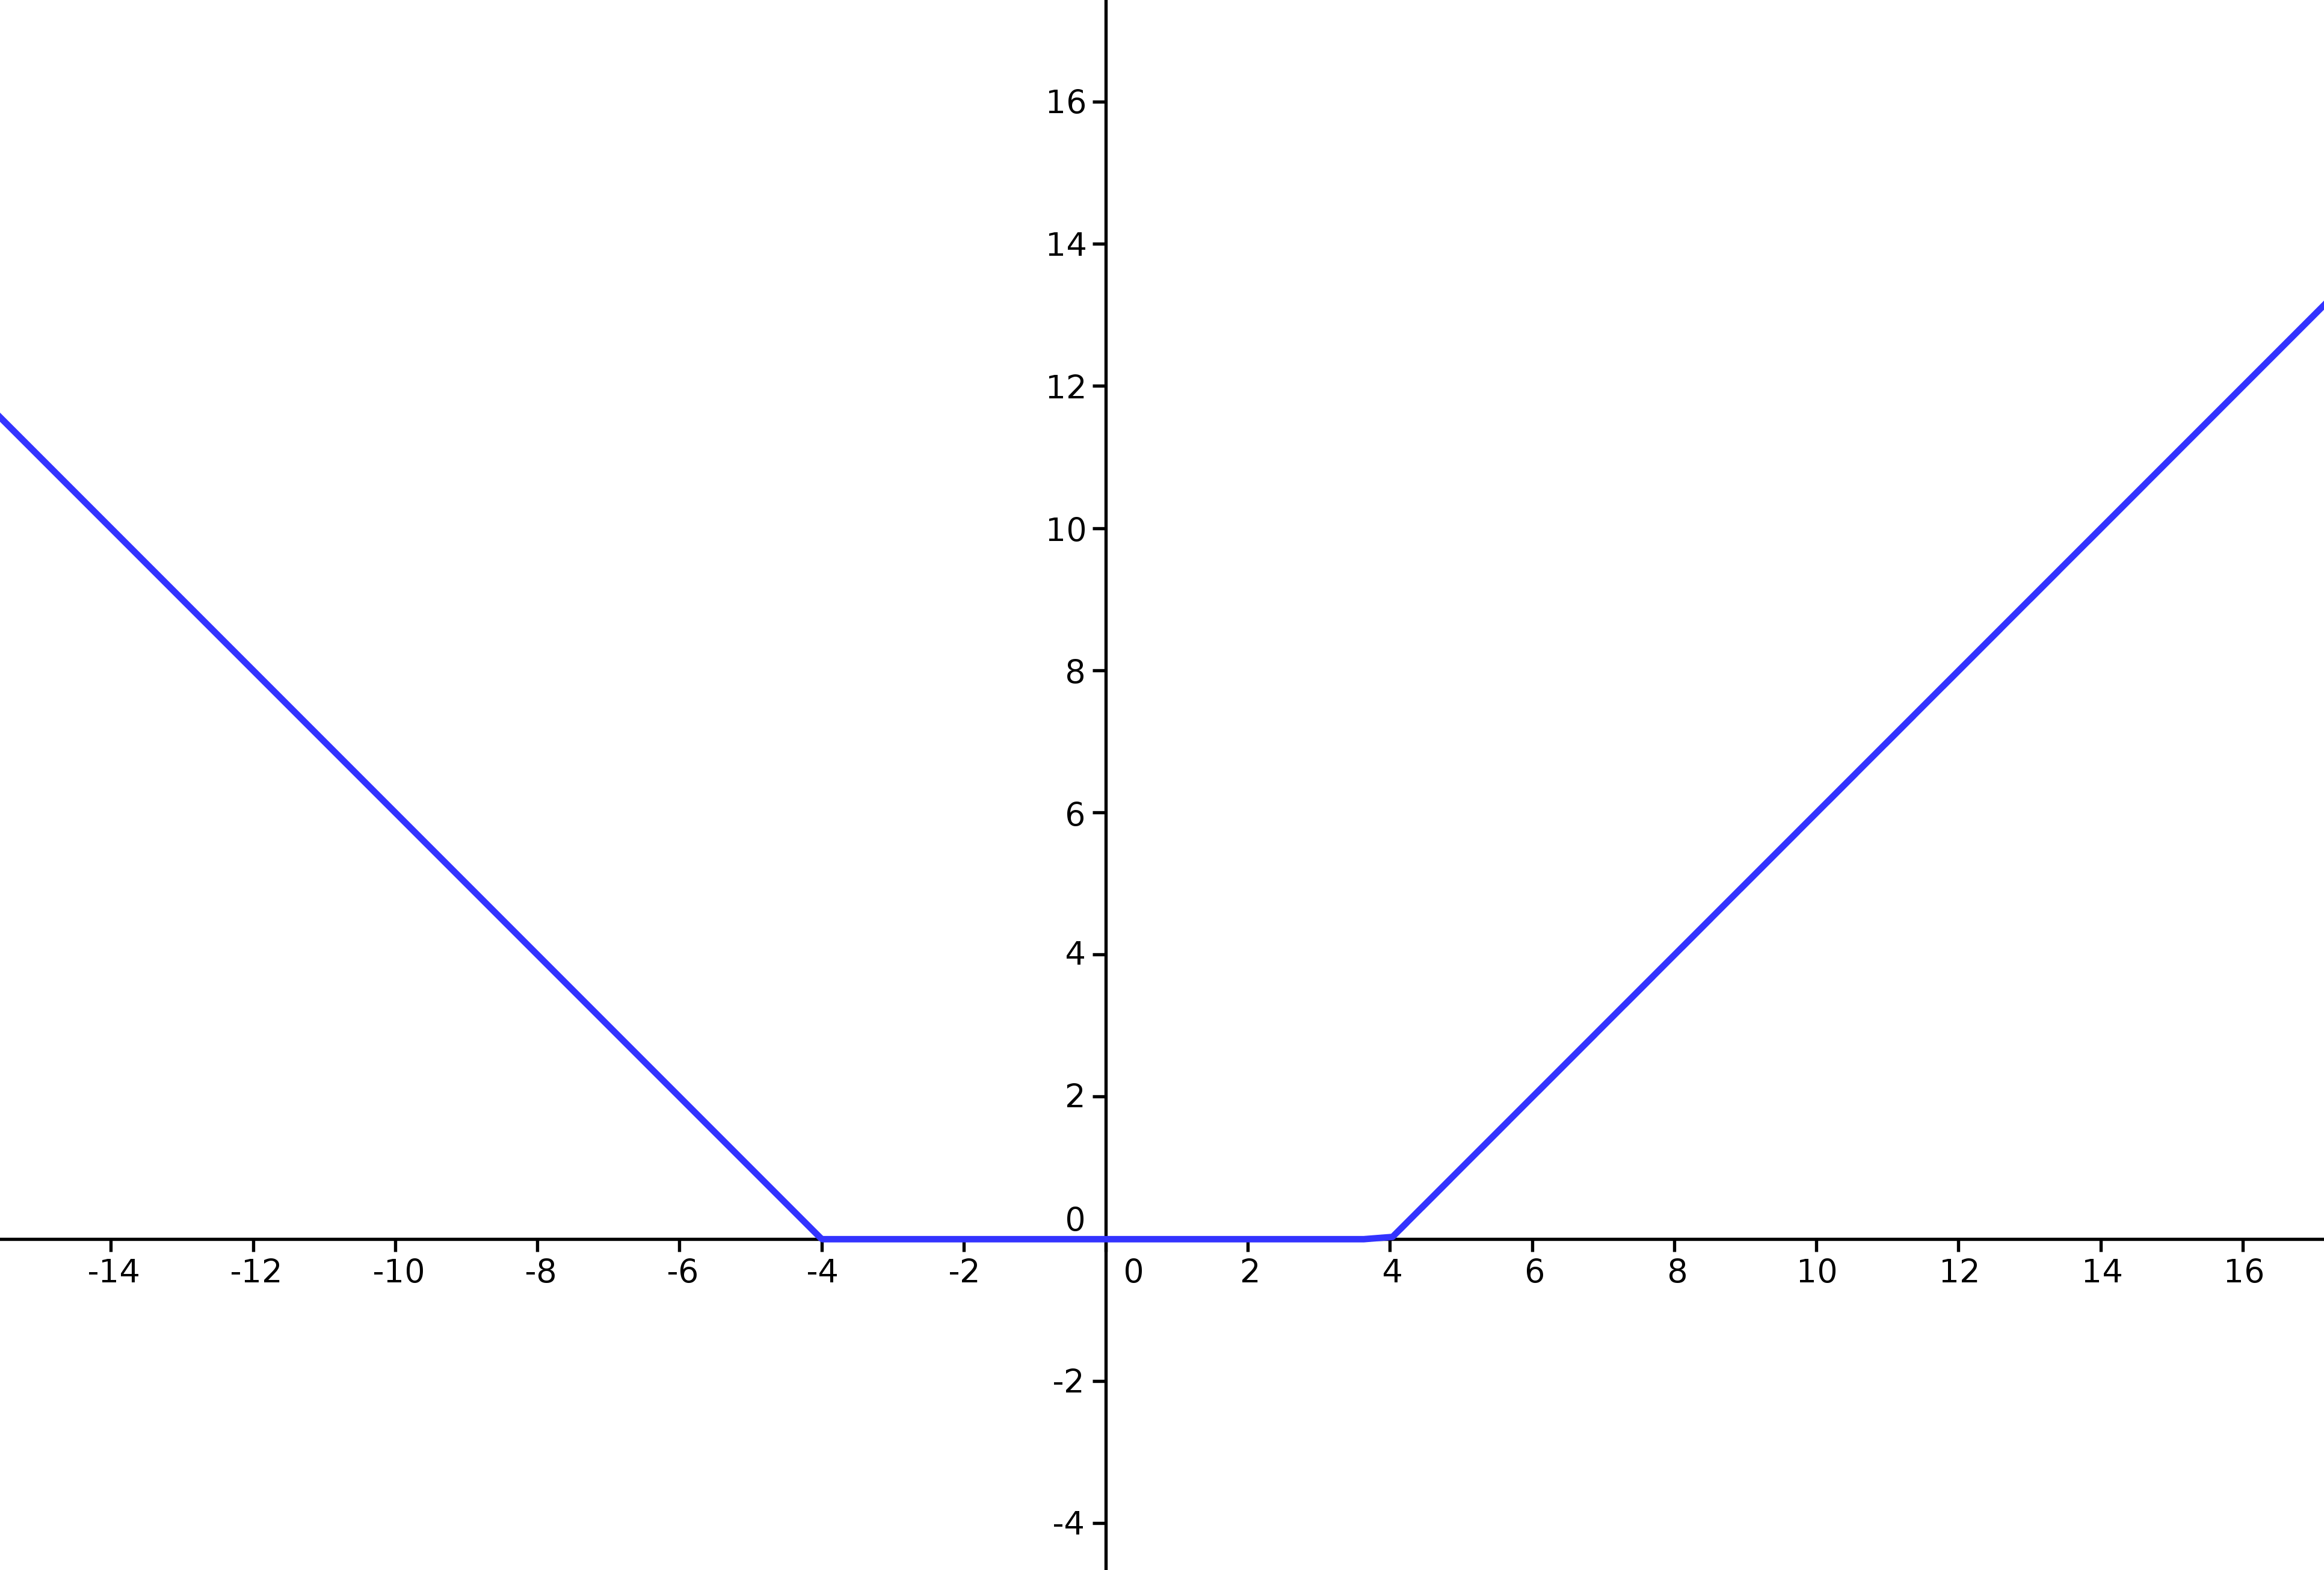
\includegraphics[width=0.5\textwidth]{assets/convex.png}
        \caption{Convex function illustration}
    \end{figure}
    \item Even if it is not strongly convex, it has a global minimum, just not only one.
    \item \textbf{Attention:} Just being differentiable and convex doesn't mean it has a stationary point: $f(w^{t+1}) < f(w^t)$.
    \begin{figure}[h]
        \centering
        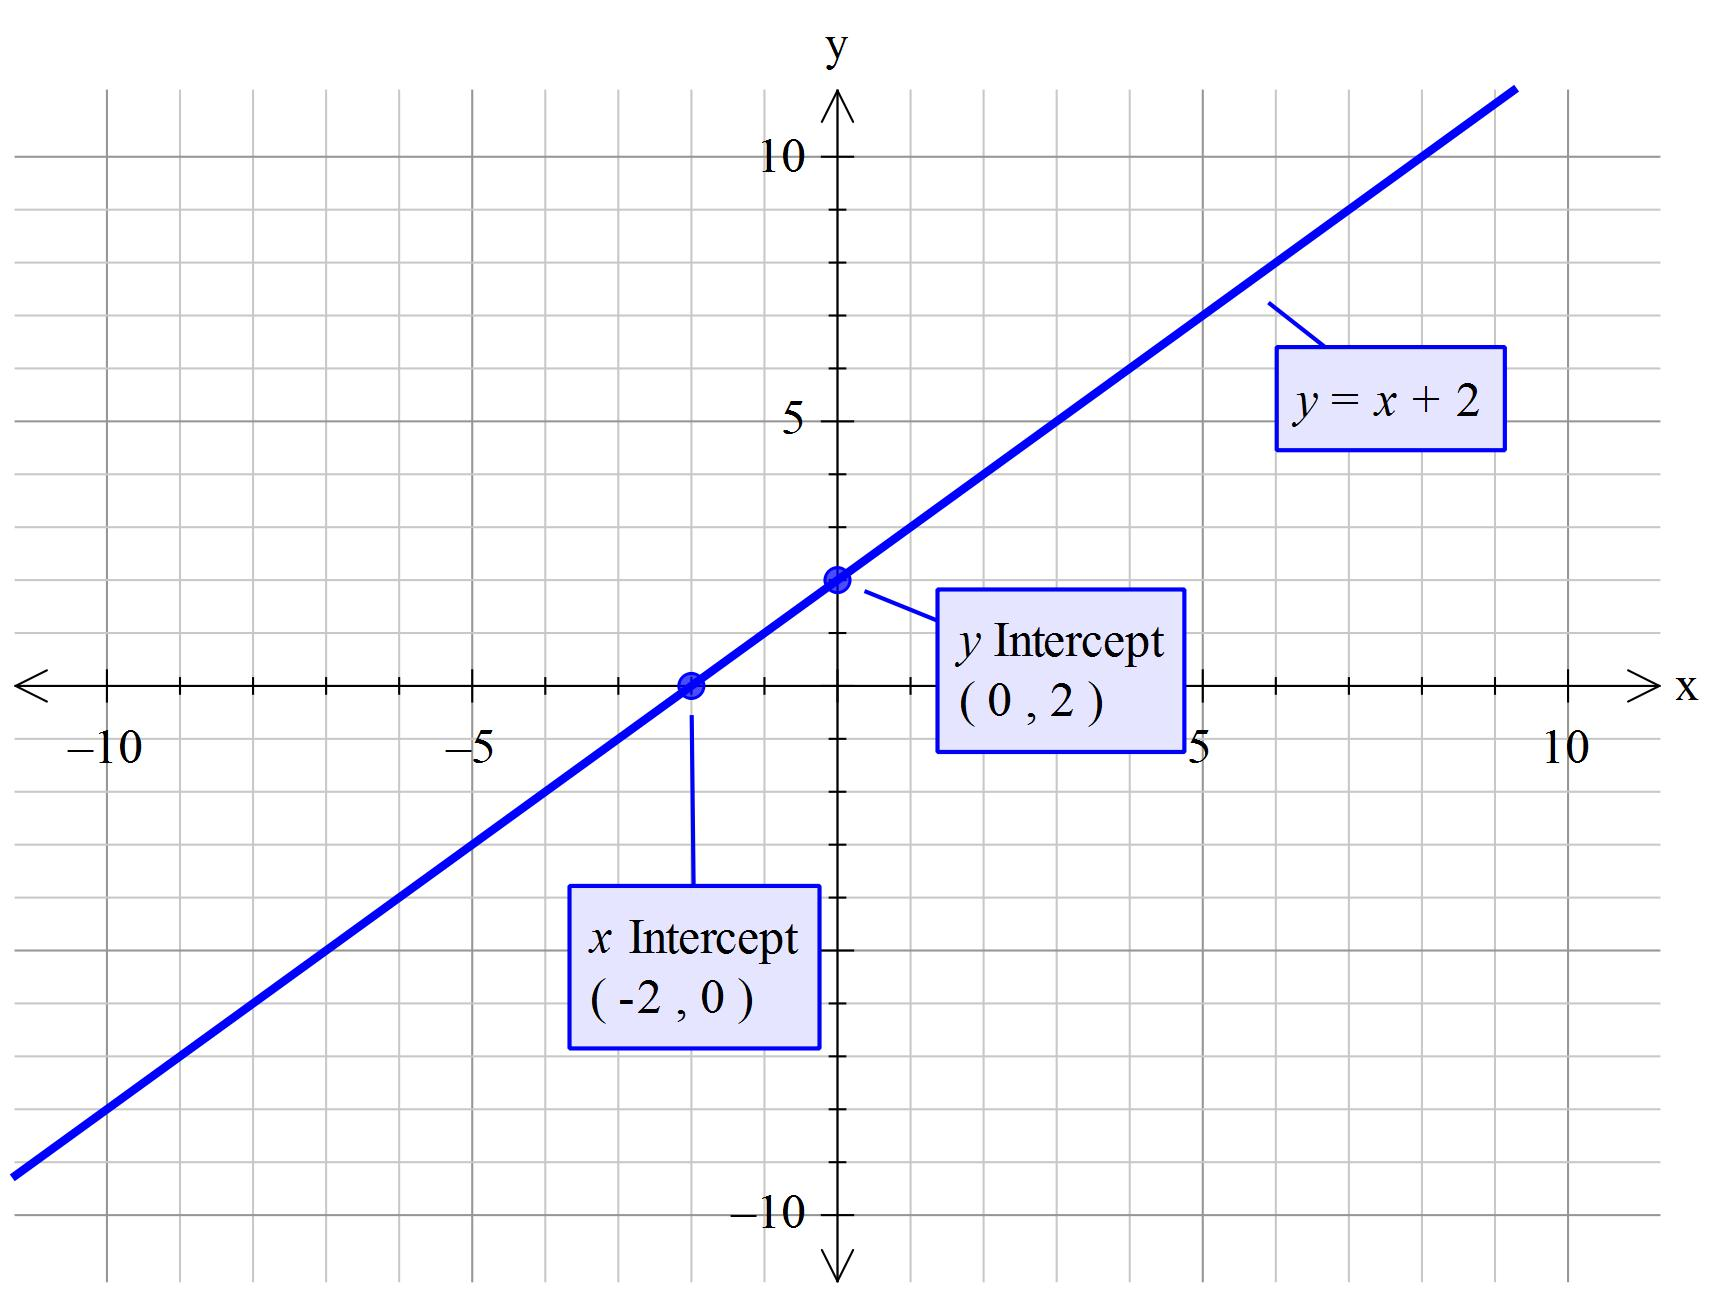
\includegraphics[width=0.5\textwidth]{assets/x.jpeg}
        \caption{Convex but has no maximum, minimum, saddle point}
    \end{figure}
    \item Only a strong convex function implies a semi-definite positive Hessian matrix.
\end{itemize}

% Gradient Descent
\section{Gradient Descent}
Consider the gradient descent algorithm for minimizing a differentiable function $f$ with iterates $w^{t + 1} = w^{t} - \eta \nabla f(w^t)$. Suppose that $||\nabla f(w^t)|| > 0$. Then there always exists a step-size $\eta > 0$ such that.

\textbf{Attention:} This is only the case for gradient descent and not stochastic gradient descent!

% Discriminative vs Generative Models
\section{Discriminative vs Generative Models}
\begin{figure}[h]
    \centering
    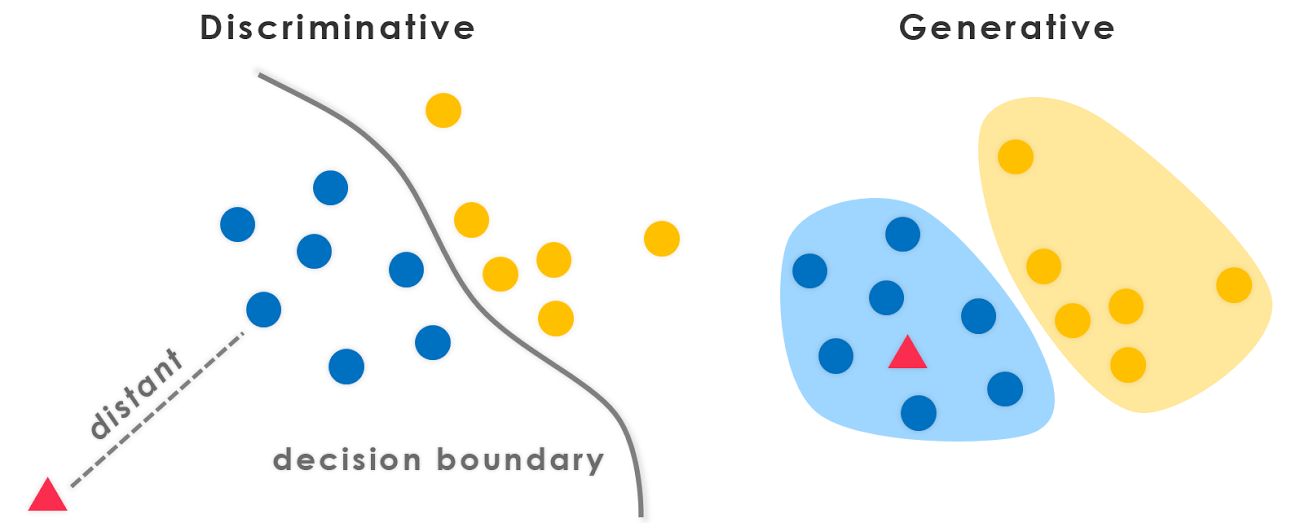
\includegraphics[width=0.7\textwidth]{assets/dis_vs_gen.png}
    \caption{Difference between discriminative and generative models}
\end{figure}

\begin{center}
\begin{tabular}{|l|l|l|}
\hline
\textbf{Description} & \textbf{Discriminative} & \textbf{Generative} \\
\hline
What is modeled & $P(y \| x)$ & $P(x, y)$ \\
What is learned & Decision boundary & Probability distribution of data \\
Example & SVM, logistic regression & Gaussian Bayes classifier, GANS \\
Advantage & Cheaper, less prone to overfitting & Good at detecting outliers, generate new data \\
\hline
\end{tabular}
\end{center}

% Gaussian Bayes Classifier (GBC)
\section{Gaussian Bayes Classifier (GBC)}
\textbf{How is $P(x, y)$ modeled?}
\begin{align*}
P(x, y) &= P(y) \cdot P(x | y) \\
P(Y = y) &= \text{Categorical Distribution} \\
P(X = x | Y = y) &= \text{XI}(x; M_y, \sum_y)
\end{align*}

% Convolutional neural network (CNN)
\section{Convolutional Neural Network (CNN)}
A convolutional neural network consists of an input layer, hidden layers, and an output layer. In a CNN, the hidden layers include one or more layers that perform convolutions.

In a CNN, the input is a tensor with shape: (number of inputs) × (input height) × (input width) × (input channels). After passing through a convolutional layer, the image becomes abstracted to a feature map, also called an activation map, with shape: (number of inputs) × (feature map height) × (feature map width) × (feature map channels).

\[
\text{Parameters} = K \times K \times K \times C \times F
\]

A higher threshold leads to fewer positive predictions, reducing the false positive rate for higher thresholds.

% Ridge Regression
\section{Ridge Regression}
\begin{itemize}
    \item Has increased bias for decreased variance.
    \item Closed form: $w^{\text{ridge}}(\lambda) = (X^TX + \lambda I^d)^{-1}X^Ty$
    \item Has very low weighted values.
    \item Regularization tries to keep weights small.
\end{itemize}

% Lasso Regression
\section{Lasso Regression}
\begin{itemize}
    \item Has no closed-form solution.
    \item Has zero values.
\end{itemize}

% Ordinary Least Squares
\section{Ordinary Least Squares}
\begin{itemize}
    \item Augmenting the set of features used for the regression will never increase the least squares loss.
    \item Subtracting the empirical mean from the data before performing regression on the centered samples.
\end{itemize}

% SVM
\section{Support Vector Machine (SVM)}
\begin{itemize}
    \item Support vectors are the closest to the boundary.
    \item Unconstrained soft-margin SVM is an $l_2$-penalized hinge loss.
    \begin{figure}[h]
        \centering
        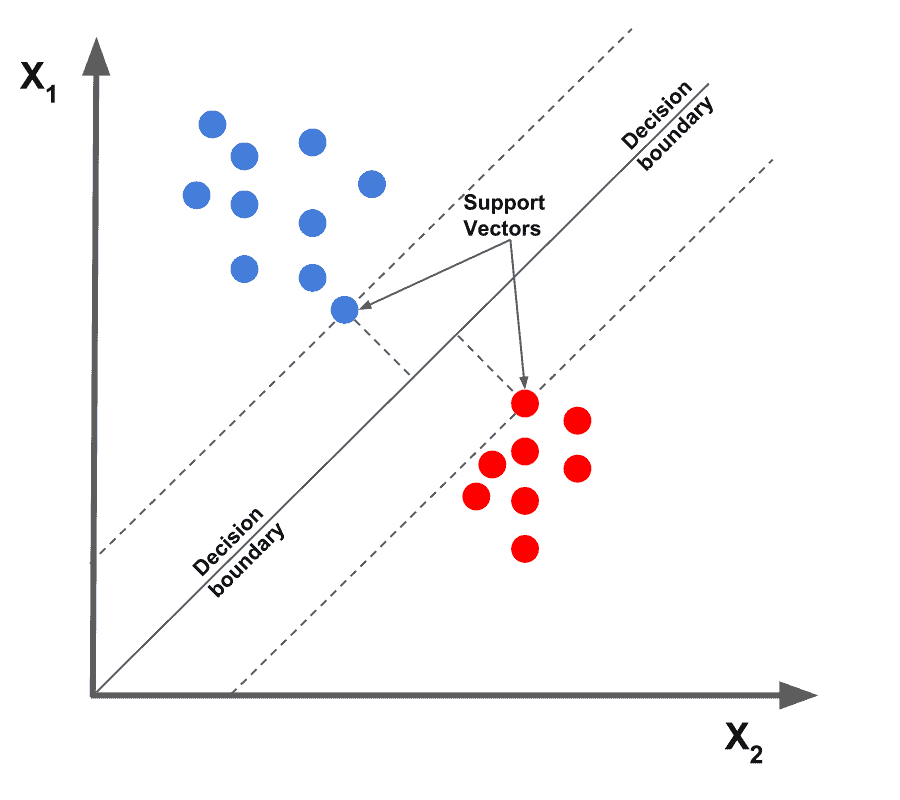
\includegraphics[width=0.5\textwidth]{assets/svm.png}
        \caption{Support Vector Machine}
    \end{figure}
\end{itemize}

% EM algorithm
\section{Expectation-Maximization (EM) Algorithm}
\begin{itemize}
    \item EM algorithm converges to a local maximum/saddle point, not only with careful initialization.
    \item Every iteration of the EM algorithm increases the marginal likelihood of the data.
    \item Instead of the EM algorithm, it is possible to adapt gradient descent for learning the parameters of the GMM and its latent assignments.
    \item Doesn't have step size.
    \item Iterative optimization algorithm used to estimate the parameters of probabilistic models when some data is missing or unobserved.
\end{itemize}

% Gaussian Mixture Model
\section{Gaussian Mixture Model}
\begin{itemize}
    \item Probabilistic model used for representing complex data distributions.
    \item Works well when data is believed to be generated from a mixture of Gaussian distributions.
    \item Parameters of GMM:
    \begin{itemize}
        \item Means: Represent the center of each component.
        \item Covariance: Controls the shape and orientation of the component.
        \item Mixing coefficients: Relative contribution of each component to the overall distribution.
    \end{itemize}
    \item Trained using Expectation-Maximization (EM) algorithm.
\end{itemize}

% Bootstrap
\section{Bootstrap}
\subsection{Advantage of using bootstrap parameter estimates in comparison with distribution-dependent parameter estimates}
\begin{itemize}
    \item There is no closed-form solution for bootstrap parameter estimates.
    \item Bootstrap sampling is a way of artificially creating more datasets. Basically, you take random samples from the dataset with replacement.
    \item Sampling with replacements makes it
    \item computationally expensive.
    \item Bootstrapping is possible for any ML technique, as it can be computed for any black-box predictor.
    \item Bootstrap estimates are not asymptotically stable.
\end{itemize}

% Generative Adversarial Networks
\section{Generative Adversarial Networks}
$D$: discriminator
$G$: neural network generator 
\begin{itemize}
    \item If $D$ and $G$ both have enough capacity, i.e., if they can model arbitrary functions, the optimal $G$ will be such that $G(z) \sim p_{data}$.
    \item The objective can be interpreted as a two-player game between $G$ and $D$.
    \item The output of the discriminator is the probability of classifying $x$ as being real:
    \[
    1 - D_G(x)
    \]
\end{itemize}

% Naive Bayes classifiers
\section{Naive Bayes Classifiers}
\begin{itemize}
    \item Every pair of features being classified is independent of each other.
    \item Bayes' Theorem:
    \[
    P(A|B) = \frac{P(B|A)P(A)}{P(B)}
    \]
\end{itemize}

% Error
\section{Error}
\begin{figure}[h]
    \centering
    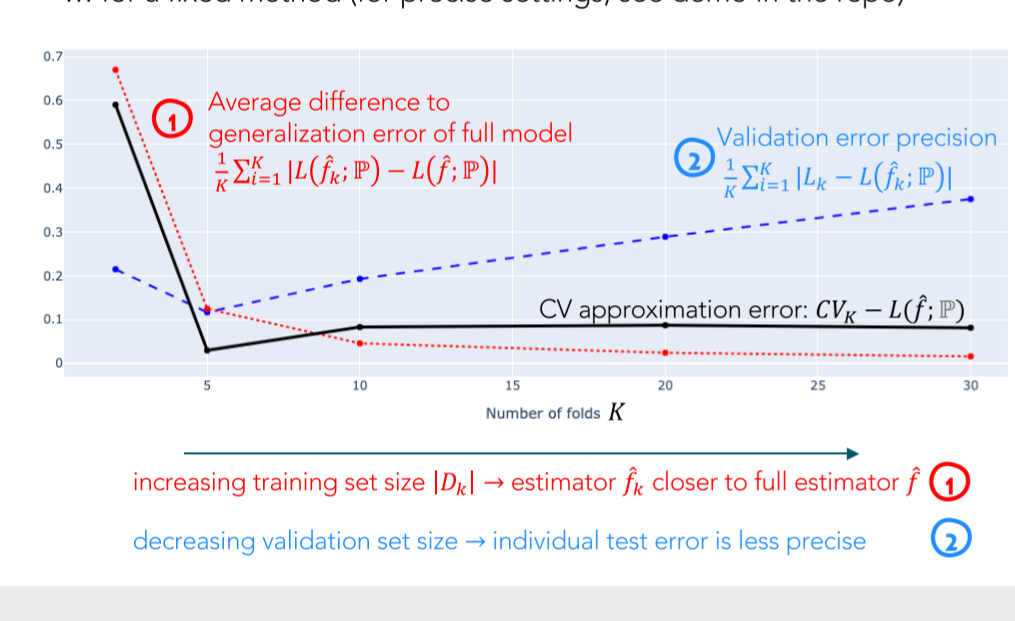
\includegraphics[width=0.5\textwidth]{assets/graph_error.png}
    \caption{Error}
\end{figure}
\begin{figure}[h]
    \centering
    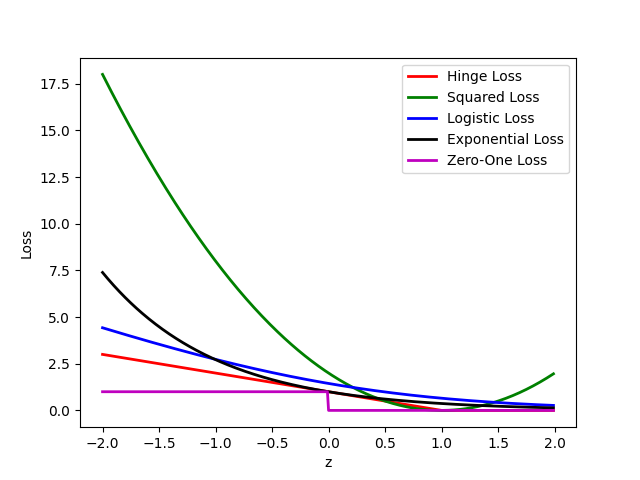
\includegraphics[width=0.5\textwidth]{assets/errors.png}
    \caption{Error types}
\end{figure}
\begin{itemize}
    \item \textbf{Logistic}: Minimum is at $\infty$.
    \item \textbf{Square}:
    \begin{itemize}
        \item Well-defined minimum, but the point is that this minimum (at 1) seems a bit random and does not make a lot of sense.
    \end{itemize}
    \item \textbf{Exponential}:
    \begin{itemize}
        \item Penalizes wrong labels very much and very quickly. Even one error could heavily penalize your model.
        \item Has exploding derivatives for wrong results and therefore is unstable.
    \end{itemize}
    \item \textbf{Hinge}:
    \begin{itemize}
        \item For SVM.
        \item Is convex.
        \item Has a minimum.
        \item Not differentiable at 1.
    \end{itemize}
    \item \textbf{Logistic}:
    \begin{itemize}
        \item For cross-entropy.
        \item Differentiable at all points.
        \item Models conditional probability $p(y | w, x)$.
        \item The logistic loss doesn't necessarily maximize the margin between classes since it takes into account all the samples in both classes.
    \end{itemize}
    \item \textbf{Linear}:
    \begin{itemize}
        \item Too sensitive to outliers and returns garbage when there is an imbalance in data.
    \end{itemize}
    \item \textbf{0-1-Loss}:
    \begin{itemize}
        \item Derivative is always 0, doesn't make sense to optimize that.
    \end{itemize}
    \item \textbf{Cross-Entropy Loss in Classification}:
    \begin{itemize}
        \item Cross-entropy loss is a crucial component in training classification models.
        \item It quantifies the dissimilarity between predicted class probabilities and actual class labels.
        \item For each data point, the cross-entropy loss is computed by taking the negative logarithm of the predicted probability assigned to the true class:
        \[
        L_i = -\sum_{k=1}^{K} y_{ik} \cdot \log(p_{ik})
        \]
        \item This loss function not only measures the correctness of the model's predictions but also encourages the model to be confident and accurate in its class probability assignments.
        \item The overall objective during training is to minimize the mean cross-entropy loss across the dataset:
        \[
        L = \frac{1}{N} \sum_{i=1}^{N} L_i
        \]
    \end{itemize}
\end{itemize}

% Asymmetric 0-1 loss with abstention
\section{Asymmetric 0-1 Loss with Abstention}
We shall define a new loss named 0-1 loss with abstention with an \textit{extended action space}:
\[
f(x) \in \{-1, +1, r\}
\]
where $r$ indicates \textbf{abstaining from a prediction}. This method is sometimes called \textbf{selective classification}. We also introduce a cost $c \in[0, 0.5]$ for abstaining. The loss becomes:
\[
l(f(x), y) = \mathbf{1}_{f(x)\neq y} \mathbf{1}_{f(x) \neq r} + c \mathbf{1}_{f(x) = r}
\]
We should abstain if:
\[
c < \min \{p(x), 1 - p(x)\}
\]
\begin{figure}[h]
    \centering
    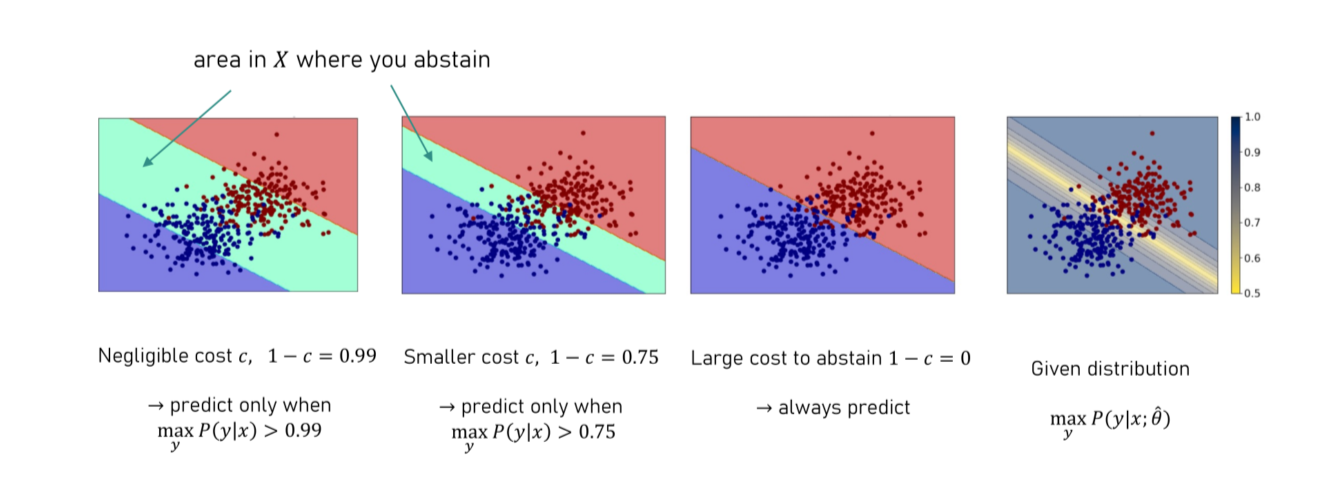
\includegraphics[width=0.7\textwidth]{assets/0-1-loss.png}
    \caption{Asymmetric 0-1 Loss with Abstention}
\end{figure}

% Classification
\section{Classification}
The margin of a decision hyperplane to be the (smallest) distance between the hyperplane and the data points. The margin of the hyperplane $\hat{w}$ is defined as $\frac{1}{||\hat{w}||}$.

% Quiz
\section{Quiz}
\subsection{K-means clustering}
\begin{itemize}
    \item Seeks cluster centers and assignments to minimize the within-cluster sum of squares.
    \item Appropriate if the underlying clusters are separable, spherical, and approximately of the same size.
    \item K-means clustering can be kernelized.
\end{itemize}

\subsection{Find k}
\begin{itemize}
    \item By using a heuristic like the elbow method that identifies the diminishing returns from increasing k.
    \item By using an information criterion that regularizes the solution to favor simpler models with lower k.
\end{itemize}

\subsection{Lloyd's algorithm}
\begin{itemize}
    \item It cannot cycle; i.e., it does never return to a particular solution after having previously changed to a different solution.
    \item Using specialized initialization schemes (e.g., k-means++) can improve the quality of solutions found by the algorithm and reduce its runtime.
    \item Center of clusters should be at the center of gravity.
    \item So after choosing centers and clustering, move centers to new centers.
    \item Repeat until done.
    \item Converges, local or global minimum.
\end{itemize}

\subsection{PCA}
\begin{itemize}
    \item PCA can be kernelized.
    \item Unsupervised learning algorithm.
    \item It is orthogonal to all other principal components found by PCA.
    \item If we use the Gaussian kernel for kernel PCA, we implicitly perform PCA on an infinite-dimensional feature space.
    \item Gaussian kernel has infinite dimensions.
    \item Autoencoders and PCA are the same thing if we choose the activation function $\varphi(\cdot)$.
    \item For every arbitrary finite dataset with two classes and distinct points, there exists a feature map $\phi$, such that the dataset becomes linearly separable.
    \begin{itemize}
        \item As long as it is finite with two datasets A, B to separate, one can literally define a feature map:
        \[
        \phi(x) = \begin{cases}
            1 & \text{if } x \in A \\
            -1 & \text{otherwise}
        \end{cases}
        \]
    \end{itemize}
\end{itemize}

\subsection{PCA first principal component}
\begin{itemize}
    \item Captures the maximum amount of variance in the data among all possible linear combinations of the original features.
    \item Represents the direction in the data space along which the data exhibits the highest variability or spread.
    \item Orthogonal to all other subsequent principal components, meaning it is uncorrelated with them. This orthogonality property allows PCA to create uncorrelated features.
    \item The first principal component is given by the eigenvector of the data covariance matrix with the largest eigenvalue.
\end{itemize}

\end{document}
